\documentclass[tikz]{standalone} 
\usetikzlibrary{arrows, decorations.markings}
\usetikzlibrary{arrows.meta}
\begin{document}

   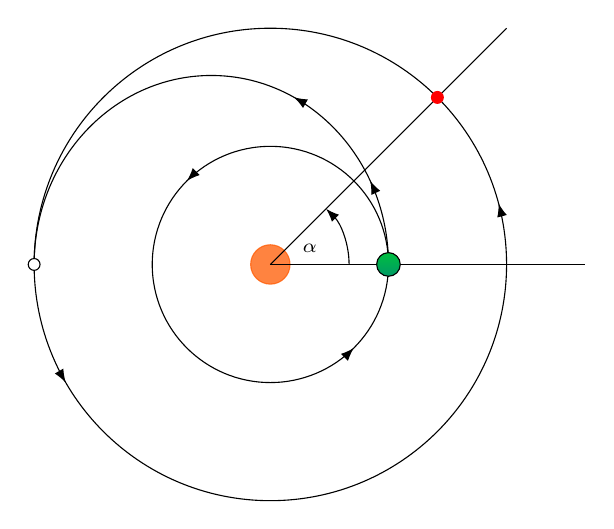
\begin{tikzpicture}[>=Latex,
                       mydeco/.style = {decoration = {markings, 
                                                       mark = at position #1 with {\arrow{>}}}
                                       }
                      ]
     \filldraw[orange!60!yellow!50!red, opacity = .75] (0,0) circle (.25cm);
     \draw (0,0) -- (4,0);
     \draw (0,0) -- (3,3);
     \draw[postaction = {mydeco=0.0416 ,decorate}, 
           postaction = {mydeco=0.58333 ,decorate}] (0,0) circle (3cm);

     \draw[postaction = {mydeco=0.375 ,decorate}, 
           postaction = {mydeco=0.875 ,decorate}] (0,0) circle (1.5cm);

     \filldraw[red] (2.12132,2.12132) circle (.075cm);
     \draw[->] (1,0) arc (0:45:1cm) 
                       node[fill = white,inner sep = .05cm] at (.5,.2) {$\scriptstyle\alpha$};


     \draw[postaction = {mydeco=0.15 ,decorate}, 
           postaction = {mydeco=0.35 ,decorate}] (0:1.5) arc (0:180:2.25cm and 2.4cm);

   \draw[fill = white] (-3,0) circle (.075cm);

   \filldraw[top color = green!75!blue, bottom color = blue!40!green] (1.5,0) circle (.15cm);

   \end{tikzpicture}

\end{document}
